%!TEX encoding = UTF-8 Unicode

\begin{IEEEbiography}[{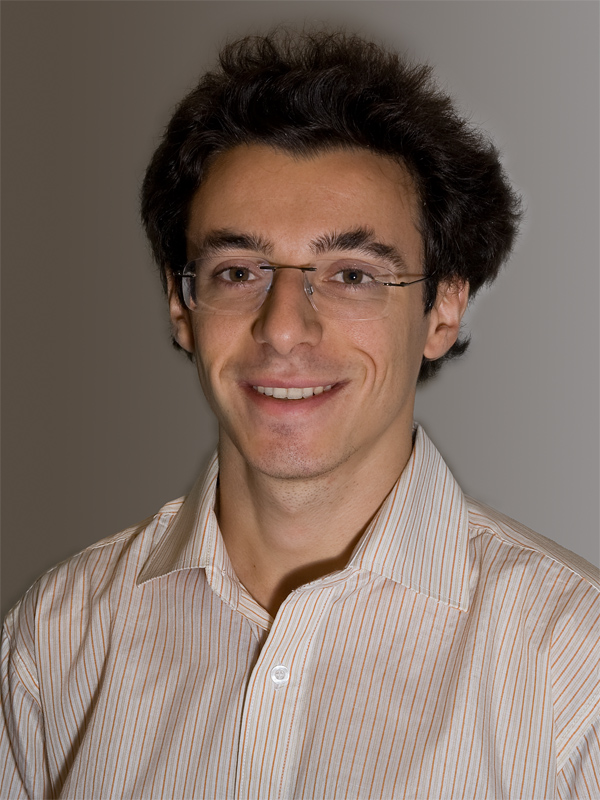
\includegraphics[width=1in,height=1.25in,clip,keepaspectratio]{./author_bios_and_photos/giovanni_saponaro}}]{Giovanni Saponaro}
  is a Ph.D. candidate at Instituto Superior Técnico (IST), Lisbon, Portugal, and a member of the local Computer and Robot Vision Laboratory (VisLab) of the Institute for Systems and Robotics. His research focuses on visual scene understanding and robot decision algorithms that support \hri{} with highly advanced humanoid robots such as the iCub, and in the presence of uncertainty. He received his M.Sc. in Computer Engineering -- \acl{AI} Systems from Sapienza University of Rome (Italy) in 2009 (with honors), and a B.Sc. in Computer Engineering from the same university in 2005. He published more than 10 papers in the diverse areas of cognitive systems, developmental robotics, visual perception of objects and of human body gestures for action recognition. He participated in the international research project POETICON++, together with linguists, computer vision experts, neuroscientists and roboticists.
\end{IEEEbiography}

\begin{IEEEbiography}[{
\includegraphics[width=1in,height=1.25in,clip,keepaspectratio]{./author_bios_and_photos/jamone_qmul_100x150px_LD}}]{Lorenzo Jamone}
  is a Lecturer in Robotics at the Queen Mary University of London (UK). He received his MS in Computer Engineering from the University of Genoa (Italy) in 2006 (with honors), and his PhD in Humanoid Technologies from the University of Genoa and the Italian Institute of Technology (IIT) in 2010. He was Associate Researcher at the Takanishi Laboratory in Waseda University (Tokyo, Japan) from 2010 to 2012, and Associate Researcher at VisLab laboratory of the Instituto Superior Tecnico (Lisbon, Portugal) from 2012 to 2016. His research interests include cognitive humanoid robots, sensorimotor learning and control, robotic manipulation, force and tactile sensing (more than 60 publications, h-index 16).
\end{IEEEbiography}

\begin{IEEEbiography}[{
\includegraphics[width=1in,height=1.25in,clip,keepaspectratio]{./author_bios_and_photos/alexandre_bernardino}}]{Alexandre Bernardino}
  (PhD 2004) is an Associate Professor at the Dept. of Electrical and Computer Engineering and Senior Researcher at the Computer and Robot Vision Laboratory of the Institute for Systems and Robotics at IST, the faculty of engineering of Lisbon University. He has participated in several national and international research projects as principal investigator and technical manager. He published more than 40 research papers in peer-reviewed journals and more than 100 papers on peer-reviewed conferences in the field of robotics, vision and cognitive systems. He is associate editor of the journal Frontiers in Robotics and AI and of major robotics conferences (ICRA, IROS). He has graduated 10 PhD students and more than 40 MSc students. He was co-supervisor of the PhD Thesis that won the IBM Prize 2014 and the supervisor of the Best Robotics Portuguese MSc thesis award of 2012. He is a Senior Member of the IEEE and the current chair or the IEEE Portugal Robotics and Automation Chapter. His main research interests focus on the application of computer vision, machine learning, cognitive science and control theory to advanced robotics and automation systems.
\end{IEEEbiography}

\begin{IEEEbiography}[{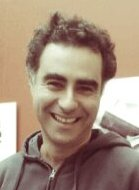
\includegraphics[width=1in,height=1.25in,clip,keepaspectratio]{./author_bios_and_photos/gsalvi}}]{Giampiero Salvi}
received the MSc degree in Electrical Engineering from Università la Sapienza (Rome, Italy) and the PhD degree in Computer Science from KTH Royal Institute of Technology (Stockholm, Sweden). He was a post-doctoral fellow at the Institute of Systems and Robotics (ISR), Lisbon, Portugal. He is currently Associate Professor in Machine Learning and Director of the Masters Programme in Machine Learning at KTH Royal Institute of Technology. His main interests are machine learning, speech technology, and cognitive systems.
\end{IEEEbiography}
